\chapter{Data}

\section{Structured paradigm data}

The English Wiktionary, a collaborative online dictionary, has become something of a standard source of supervised morphological data. It provides full or partial inflection tables alongside lexeme definitions; the structure of tables is consistent for a given language and part of speech. An example table is given in figure 3.1. For some highly inflected languages (e.g., Navajo), Wiktionary only provides a fixed subset of forms. For some relationships between words that could be considered grammatical, it may simply offer them as separate lexical entries; for example, Russian perfect and imperfect forms are given as separate entries, as are Navajo verb forms that vary by aspect or thematic classifier \parencite{Wiktionary}.  

\begin{figure}[t]
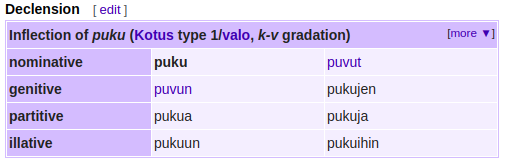
\includegraphics[width=12cm]{images/puku.png}
\centering
\caption{The English Wiktionary partial inflection table for the Finnish word \textit{puku}.}
\end{figure}

\begin{figure}[t]
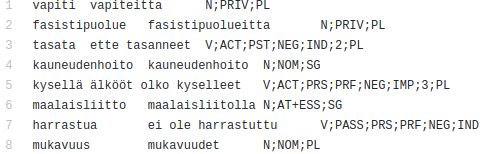
\includegraphics[width=12cm]{images/sigmorphon2018_fn.png}
\centering
\caption{A sample of the SIGMORPHON 2018 data for Finnish, scraped from Wiktionary and provided on GitHub (https://github.com/sigmorphon/conll2018/blob/master/task1/all/finnish-train-high).}
\end{figure}

Specific Wiktionary dumps have come to be used as standard datasets, used by multiple authors as a benchmark to compare model performance. \cite{Durrett2013} published a Wiktionary dataset of five paradigms from three languages (Finnish, Spanish, and German) which have been used in much future work \parencite{Hulden2014} \parencite{Nicolai2015} \parencite{Ahlberg2015} \parencite{Faruqui2015}.

SIGMORPHON 2017 published \href{https://github.com/sigmorphon/conll2017/tree/master/all}{a dataset} partitioned into three training levels (100, 1000, and 10,000 tables), containing both sparse and full inflection tables for one or more parts of speech for each of 52 languages. Most of that data was derived from a January 2017 Wiktionary dump. \parencite{Cotterell2017} 

The most complete structured dataset to date was published for the SIGMORPHON shared task 2018, a superset of the SIGMORPHON 2017 data, which is partitioned in the same manner and includes data from 103 languages. For most of the languages, data was scraped from Wiktionary. An example of some Finnish forms provided for SIGMORPHON 2018 is shown in Figure 3.2.

\section{Text corpora}

\section{Representation of morphology}

In earlier work, morphology is encoded in a language-specific and model-specific way.

\parencite{Luong2013} The UniMorph project, initially published in 2015, makes an effort to encode morphological categories uniformly cross-linguistically. \parencite{SylakGlassman2015} \parencite{SylakGlassman2015a} \parencite{SylakGlassman2016} The SIGMORPHON data since 2018 has been published in UniMorph format, seen in Figure 3.2.